\documentclass{article}

\usepackage{tikz}
\usetikzlibrary{er}

\tikzset{every node/.style={font=\itshape}}
\tikzset{total/.style={double distance=1pt}}

\author{Emily Asadoorian $\vert$ CSE-341 SP21}
\date{February 18, 2021}
\title{County Garden Insurance E-R Design Diagram}

\begin{document}

\pagenumbering{gobble}

\maketitle

\newpage

\pagenumbering{arabic}

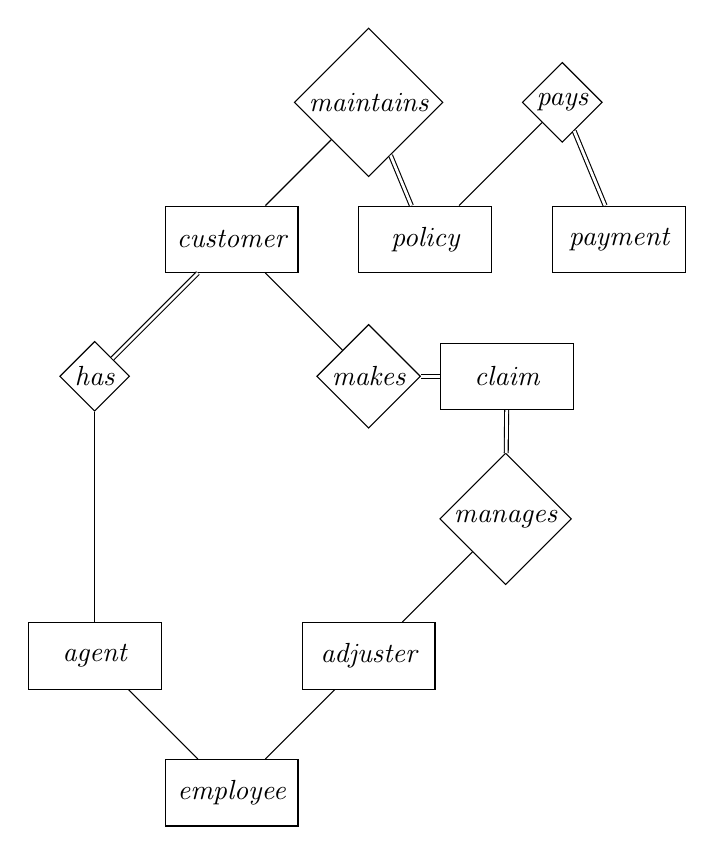
\begin{tikzpicture}[node distance=7em]

\node[entity,xshift=0.35\textwidth,yshift=-20em] (employee) {employee};
\node[entity] [above left of=employee] (agent) {agent} edge (employee);
\node[entity] [above right of=employee] (adjuster) {adjuster} edge (employee);
\node[entity,xshift=0.35\textwidth] (customer) {customer};
\node[entity] [below right of=customer,xshift=5em] (claim) {claim};
\node[entity] [right of=customer] (policy) {policy};
\node[entity] [right of=policy] (payment) {payment};

\node[relationship] [below left of=customer] (has) {has} edge[total] (customer) edge (agent);
\node[relationship] [below right of=customer] (makes) {makes} edge (customer) edge[total] (claim);
\node[relationship] [above right of=adjuster] (manages) {manages} edge (adjuster) edge[total] (claim);
\node[relationship] [above right of=customer] (maintains) {maintains} edge (customer) edge[total] (policy);
\node[relationship] [above right of=policy] (pays) {pays} edge[total] (payment) edge (policy);

\end{tikzpicture}

\end{document}
